\documentclass[a4paper,10pt]{article}

\usepackage{graphicx}
\usepackage[hmargin=1.0in,vmargin=1.00in]{geometry}
%\usepackage{pslatex}
\usepackage{setspace}
\usepackage{graphicx}
\usepackage{hyperref}
\usepackage{amssymb}
\usepackage{epstopdf}
\usepackage{listings}
\usepackage{color}
\usepackage{amsmath}
\usepackage{tikz}
\usepackage{mathtools}
\doublespacing

\title{Topological Defects in Two-Dimensional Crystals}
\author{James Antonaglia}
\date{12/08/14}

%Equations/Entries
\newcommand{\beq}{\begin{equation}}
\newcommand{\bequo}{\begin{quotation}}
\newcommand{\beqa}{\begin{eqnarray}}
\newcommand{\eeq}{\end{equation}}
\newcommand{\leeq}[1]{\label{#1}\end{equation}}
\newcommand{\equo}{\end{quotation}}
\newcommand{\eeqa}{\end{eqnarray}}
\newcommand{\non}{\nonumber}
\newcommand{\mx}{\mbox}
\newcommand{\mxf}[1]{\mbox{\footnotesize{#1}}}
\newcommand{\lb}{\label}
\newcommand{\fr}[1]{(\ref{#1})}
\newtheorem{entry}{}[section]
\newcommand{\bent}[1]{\vspace*{-2cm}\hspace*{-1cm}\begin{entry}\lb{e{#1}}\rm}
\newcommand{\eent}{\end{entry}}
\newcommand{\fre}[1]{{\bf\ref{e{#1}}}}
\newcommand{\Emark}{$\sqcap\hspace{-2.7mm}\sqcup$}
\newcommand{\sEmark}{{\fns $\sqcap\hspace{-2.3mm}\sqcup$}}
\newcommand{\fn}{\footnote}


%Greek Letters
\renewcommand{\a}{\alpha}
\renewcommand{\b}{\beta}
\newcommand{\g}{\gamma}
\newcommand{\G}{\Gamma}
\renewcommand{\d}{\delta}
\renewcommand{\th}{\theta}
\renewcommand{\k}{\kappa}
\newcommand{\Th}{\Theta}
\newcommand{\D}{\Delta}
\newcommand{\e}{\epsilon}
\newcommand{\ep}{\varepsilon}
\newcommand{\s}{\sigma}
\renewcommand{\S}{\Sigma}
\newcommand{\w}{\omega}
\newcommand{\W}{\Omega}
\newcommand{\al}{\alpha}
\newcommand{\bet}{\beta}
\newcommand{\gam}{\gamma}
\newcommand{\lam}{\lambda}
\newcommand{\Lam}{\Lambda}
\newcommand{\eps}{\varepsilon}
\newcommand{\ichi}\sichi
\renewcommand{\ni}{\sni}
\renewcommand{\r}{\rho}
\renewcommand{\t}{\tau}
\newcommand{\ph}{\varphi}
\newcommand{\sichi}{{\mbox{{\footnotesize I}}}}
\newcommand{\sni}{{\mbox{{\footnotesize II}}}}

%color2010/6/9
\newcommand{\red}{\color{red}}
\newcommand{\blue}{\color{blue}}
\newcommand{\green}{\color{green}}
\definecolor{gray}{rgb}{0.5, 0.5, 0.5}
\newcommand{\gray}{\color{gray}}

%Derivatives
\newcommand{\pder}[2]{\frac{\partial {#1}}{\partial {#2}}}
\newcommand{\pdert}[2]{\frac{\partial^2 {#1}}{\partial {#2}^2}}
\newcommand{\fder}[2]{\frac{\delta {#1}}{\delta {#2}}}
\newcommand{\PDD}[3]{\left.\frac{\partial^{2}{#1}}{\partial{#2}^{2}}\right|_{#3}
}
\newcommand{\PD}[3]{\left.\frac{\partial{#1}}{\partial{#2}}\right|_{#3}}
\newcommand{\der}[2]{\frac{d {#1}}{d {#2}}}

\renewcommand{\deg}{^\circ}
\newcommand{\com}{{\bf [C] }}
\newcommand{\cend}{\Emark\[\]\vspace*{-1. cm}}
\newcommand{\x}{\times}

%My commands
\newcommand{\win}{\ddot\smile}
\newcommand{\lose}{\ddot\frown}
\newcommand{\avg}[1]{\left \langle #1 \right \rangle}
\newcommand{\E}[1]{\ensuremath{\times10^{#1}}}
\newcommand{\abs}[1]{\ensuremath{\left | #1 \right |}}
\newcommand{\paren}[1]{\left(#1\right)}
\newcommand{\recip}[1]{\frac{1}{#1}}
\newcommand{\ex}[1]{\mathbb{E}[#1]}
\newcommand{\bprob}[1]{\textbf{#1~---}}
\newcommand{\unitv}[1]{\ensuremath{\mathbf{\hat{e}}_{#1}}}
\newcommand{\goto}{\rightarrow}
\newcommand{\expct}[1]{\mathbb{E}[#1]}
\newcommand{\mtrx}[1]{\begin{matrix}#1\end{matrix}}
\newcommand{\pmtrx}[1]{\paren{\begin{matrix}#1\end{matrix}}}
\newcommand{\cosp}[1]{\cos{\paren{#1}}}
\newcommand{\sinp}[1]{\sin{\paren{#1}}}
\newcommand{\tanp}[1]{\tan{\paren{#1}}}
\newcommand{\half}[1]{\frac{#1}{2}}
\newcommand{\ham}{\mathcal{H}}
\newcommand{\tr}{\mathrm{Tr}}
\newcommand{\bv}[1]{\mathbf{#1}}
\newcommand{\Der}[2]{\frac{d#1}{d#2}}
\renewcommand{\Dot}[2]{\ensuremath{\bv{#1}\cdot\bv{#2}}}
\newcommand{\Cross}[2]{\ensuremath{\bv{#1}\times\bv{#2}}}
\newcommand{\del}{\ensuremath{\partial}}
\newcommand{\R}{\ensuremath{\bv{r-r'}}}
\newcommand{\aR}{\ensuremath{\abs{\R}}}
\newcommand{\br}{\ensuremath{\bv{r}}}
\newcommand{\impl}{\ensuremath{\quad \Rightarrow \quad}}
\renewcommand{\div}[1]{\nabla \cdot \bv{#1}}
\newcommand{\curl}[1]{\nabla \times \bv{#1}}
\newcommand{\lapl}{\nabla^2}
\newcommand{\vint}{\int d^3r}
\newcommand{\oocs}{\recip{c^2}}
\newcommand{\mnfp}[1]{\frac{\mu_0 #1}{4\pi}}
\renewcommand{\iiint}{\int_{-\infty}^{\infty}}
\newcommand{\tpi}[1]{\paren{2\pi}^{#1}}
\newcommand{\ootpi}[1]{\recip{\paren{2\pi}^{#1}}}

\begin{document}
 
\maketitle

\begin{abstract}
 Crystal lattices break continuous translational symmetry, and thus they 
exhibit Goldstone modes, namely phonons. In three or more dimensions, long 
range order is robust, but crystals in two or fewer dimensions do not possess 
long range order (at $T>0$) because long-wavelength phonons destroy 
long-range correlations. In precisely two dimensions, crystals exhibit 
\emph{quasi-long range order}, with spatial correlations that decay as a power 
law in distance, and they still exhibit solid-like properties like 
nonzero elastic 
shear moduli. However, as the temperature is increased from 0, two-dimensional 
crystals exhibit \emph{topological} excitations that destroy local 
translational order. This paper is meant to be a rudimentary 
introduction to the phenomena of topological defects in two-dimensional 
lattices.
\end{abstract}

\pagebreak

\section{Topological Excitations in the XY Model}
One of the simplest and most well-studied two-dimensional system that exhibits 
a phase transition is the XY model for planar magnetism. The model consists of 
a latice of spins that can take on continuous values $(S_x,S_y)$ such that 
$\abs{\bv{S}} \leq 1$. The ferromagnetic model energetically penalizes 
neighboring spins that are misaligned. If only nearest neighbor couplings are 
considered, then the Hamiltonian is
\beq \mathcal{H} = -J \sum_{\left \langle i,j \right \rangle} \bv S_i \cdot 
\bv S_j = -J \sum_{\left \langle i,j \right \rangle} \abs{\bv S_i}\abs{\bv 
S_j}\cos\paren{\th_i - \th_j}.\eeq
The ground state of the system is where all spins have magnitude 1 and point 
along the same direction. This phase breaks global rotational invariance, so, 
by Goldstone's theorem, we should expect an elementary excitation 
associated with this broken symmetry. This is the spin-wave, which is a spatial 
modulation in the spins' orientations. The lowest order approximation expands 
the cosine term to the first nontrivial term and posits that $\abs{\bv S_i} 
= 1$:
\beq \mathcal{H} = -\frac{J}{2k_BT}\sum_{\left \langle i,j \right \rangle} 
\paren{\th_i-\th_j}^2. \eeq
This low-temperature approximation is solvable by moving to Fourier 
space. I report here the results 
from Jos\'e et al.~\cite{Jose}, where the authors calculate the spin-spin 
correlation function for a square lattice and large separation distances:
\beq \avg{\Dot{S_i}{S_j}} = \mathrm{Re}\left[\avg{e^{i(\th_i-\th_j)}}\right ] 
\sim r_{ij}^{-\eta(T)}, \qquad \eta(T) = \frac{k_BT}{2\pi J}. \eeq
Here, $r_{ij}$ is the separation distance between the spins, and $\eta$ is a 
non-universal exponent that depends on the temperature and the spin coupling 
$J$, with a more detailed calculation available in the appendix. This result is 
consistent with the Mermin-Wagner theorem \cite{MerminWagner}, which states for 
continuous spin system in two or fewer dimensions, there is no long range order 
(LRO). LRO would manifest as a constant-valued correlation function for all 
values of $r_{ij}$. In one dimension, the situation is even worse, where the 
correlation function decays exponentially for all temperatures.

From this low-temperature approximation, it seems that the correlations decay 
faster and faster for all temperatures, but it is reasonable to expect that 
other important physics that were thrown away in the quadratic approximation 
will come into effect as the temperature increases. The most important 
consequence is that the quadratic approximation violates the periodicity 
symmetry of the spin variable $\th_i$. The system is clearly invariant under 
$\th_i \goto \th_i + 2\pi n_i$, where $n_i$ is an integer-valued field on the 
lattice, which is implicitly preserved in the cosine Hamiltonian. The quadratic 
approximation ignores \emph{vortex configurations}, where a continuous closed 
path traced through the system finds that the spin variable has changed by an 
integer multiple of $2\pi$. An illustration of such defects are shown in Figure 
\ref{vortices}.

\begin{figure}
 \centering
 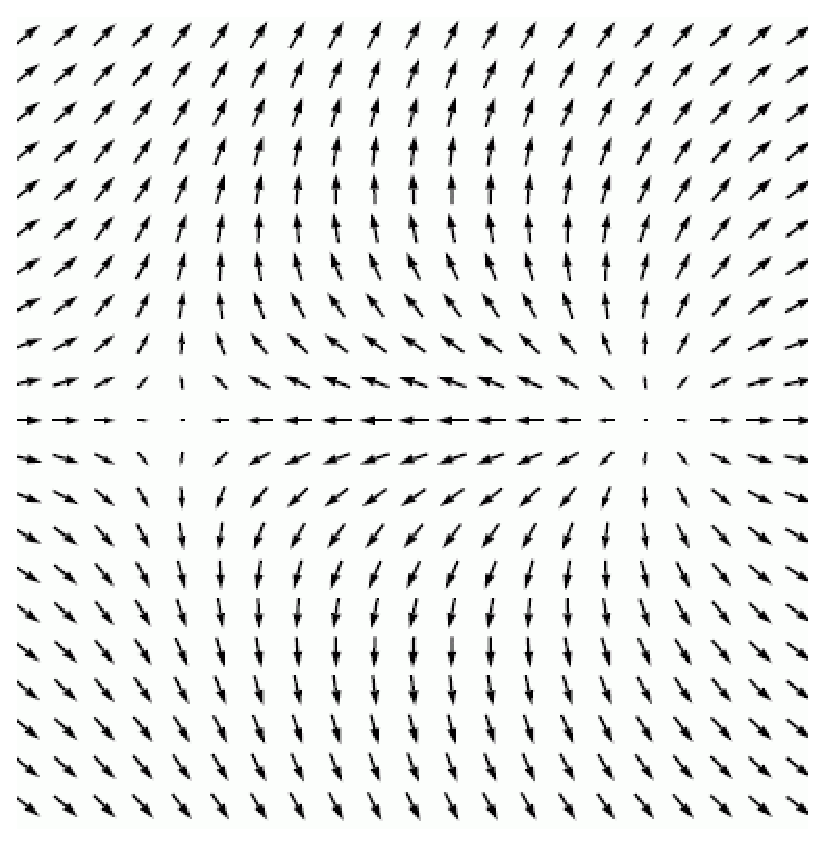
\includegraphics[scale=0.4]{vortices4.eps}
 \caption{The left defect is a vortex with winding number 1, and the 
right defect is an antivortex, or a vortex with winding number -1. Image credit 
to \url{http://www.ibiblio.org/e-notes/Perc/xy.htm}}
\label{vortices}
\end{figure}

The work of Kosterlitz, Thouless, and Berezinskii showed that there is a 
non-zero temperature where the correlation function switches from power-law 
decay to exponential decay \cite{KT}. Though the spin waves are responsible for 
the lack of long-range order, it is the vortices that are responsible for the 
phase transition. Below $T_C$, vortices are bound tightly in pairs of zero 
vorticity. This is because a bare vortex costs an amount of energy proportional 
to the log of the system size, so only vorticity-zero configurations are 
thermodynamically probable in the thermodynamic limit when the system size 
goes to infinity. Above $T_C$, vortices unbind and move freely about and 
destroy local order.

Vortices become important at higher temperatures where the low-temperature 
expansion is invalid, because the low-temperature expansion ignores the 
topology of the \emph{order parameter space.} The thermodynamic ground state of 
the XY system is degenerate: the spins point along a preferred direction, and 
so the average spin is a 2-d vector on the unit circle, as shown schematically 
in Figure \ref{OPspace}. A path in this order parameter space can wind around 
the space zero times, once, twice, etc., and all of these paths must be 
accounted for in any representation of the Hamiltonian. Berezinskii's solution 
was to amend the lattice Hamiltonian by including a new integer-valued field 
\cite{Berezinskii}:
\beq \mathcal{H} = -\frac{J}{2} \sum_{\left \langle i,j \right \rangle} 
\paren{\th_i - \th_j - 2\pi n_{ij} }^2, \quad n_{ij} 
\in \mathbb{Z}.\eeq

\begin{figure}
 \centering
 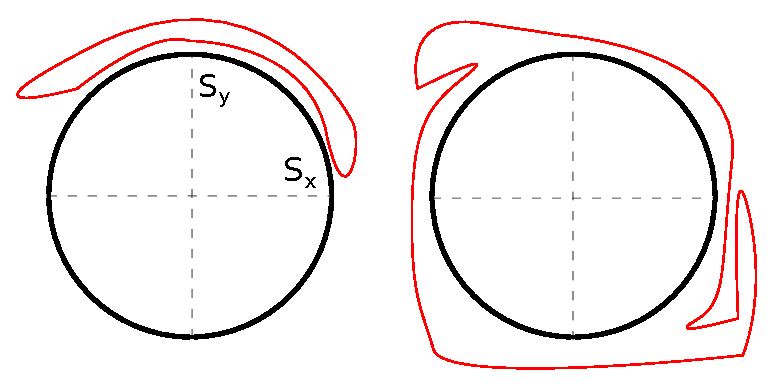
\includegraphics[scale=0.75]{topologicalspace.eps}
 \caption{The order parameter $\bv S$ lives on the unit disk (black). If a 
closed path is drawn in the system, the variable $\bv S$ changes and traces 
out a path in this order parameter space (red). The diagram on the left 
represents the loop in order parameter space where the loop in real space does 
not encircle a vortex. The loop on the right, however, represents a path in 
real space that encircles a vortex core of unit strength.}
\label{OPspace}
\end{figure}

However, a more common approach is to use a continuum model to estimate from 
macroscopic elastic constants (the Lam\'e coefficients) the energy cost of 
having a vortex in the system. Then the Hamiltonian is broken up into a 
nonsingular spin-wave part and a contribution from the quantized vortices. 
I outline here Chaikin and Lubensky's derivation \cite{Chaikin}. In the 
continuum limit, the Hamiltonian of the system is
\beq \mathcal{H} = -\half{J}\sum_{\left \langle i,j \right \rangle} 
\cos\paren{\th_i - \th_j} \goto \half{J} \int d^2\bv r \, 
\paren{\nabla \th}^2.\eeq
This is also a quadratic order approximation, so we need to put the 
vortices back in by hand. Taking a functional derivative, we find that the 
condition that minimizes the energy is Laplace's equation: $\nabla^2\th(\bv r) = 
0$. If we want to stick a single vortex with strength (winding number) $k$ into 
the system, we impose the winding condition $\oint d\bv \ell \cdot \nabla \th = 
2\pi k$ around the origin (we can put the vortex anywhere, so may as well be 
the origin). The solution is given by $\th(\br) = k\phi$, where $\phi$ is the 
polar angle in two dimensions. We have that $\nabla\phi = \recip{r} \hat{r}$, so 
the energy of the isolated vortex is
\beq E_k = \frac{J}{2} \int d^2\br \paren{\frac{k^2}{r^2}} = \pi 
Jk^2 \int_\a^R \frac{r dr}{r^2} = \pi J 
k^2\log\frac{R}{\a}.\eeq
The energy of the vortex will hit an infrared divergence unless we cut off 
the size of the system to the scale $R$, and the integral has an ultraviolet 
cutoff $\a$ which is the core radius of the vortex. This justifies the earlier 
claim that isolated vortices don't occur with any probability in the 
thermodynamic limit. The energy of a pair of vortices is calculated by linearly 
superimposing solutions to Laplace's equation and finding the energy with 
vortices of strength $k_1$ and $k_2$ separated by a distance $r$. Simply stating 
the result:
\beq E_{k_1,k_2} = \pi J \paren{k_1+k_2}^2 \log\frac{R}{\a} + 
2\pi Jk_1k_2 \log \frac{r}{\a}. \eeq
There is still the divergent term that goes as $\log R$, but if $k_1+k_2 = 0$, 
that is, if the system has no net vorticity, then the energy is 
finite. It's an interesting point that this Hamiltonian is the same as that of 
a 2-dimensional Coulomb gas, which isn't surprising because this energy was 
obtained by solving Laplace's equation in two dimensions with point 
singularities. Vortices of opposite sign are drawn together while vortices of 
like sign are pushed apart.
There is also a core energy $E_c$ which Chaikin and Lubensky calculate by 
treating $\a$ as a variational parameter. The core energy should go as 
$\a^2$, because it should be proportional to the area of the vortex. Thus the 
total energy should obey
\[ \pder{E_v}{\a} = \pder{}{\a}\paren{E_k + E_c} = \pder{}{\a}\paren{E_k + 
\a^2E_{c,0}} = 0, \quad \goto \quad \frac{\pi J k^2}{\a} = 2 E_{c,0}\a.\]
\beq \a^2 = \frac{\pi J k^2}{2 E_{c,0}},\quad E_c = \frac{\pi J 
k^2}{2}.\eeq
This is the cost of having a vortex of strength $k$, so the final Hamiltonian, 
with vortices included, is
\beq \mathcal H = \frac{J}{2}\int d^2\br \, \paren{\nabla \th}^2 + 
2\pi J\sum_{i<j} k_ik_j \log{\frac{r_{ij}}{\a} } + \frac{\pi 
J}{2}\sum_i k_i^2. \eeq
Here, all of the multi-valued nature of the field $\th(\br)$ has been removed 
and placed into the vortex terms. From this point, there are a few techniques 
to perform renormalization group calculations of fixed points for this 
Hamiltonian, but the purpose of introducing the XY model was to give a solid 
and physically intuitive picture that transfers very easily to two-dimensional 
crystals.

\section{Crystals and Hexatics in 2D Solids}
The story for a two-dimensional crystal proceeds along a similar route to the 
XY model. There is a quadratic Hamiltonian which is good to lowest order, but 
the lowest order approximation neglects topological excitations that arise 
because of the topological structure of the order parameter space. The relevant 
topological defects in a two-dimensional system are \emph{dislocations} which 
disrupt translational order and \emph{disclinations} that disrupt orientational 
order.

I will present relevant specific calculations from Nelson \cite{Nelson} and 
Jos\'e \cite{40years}. The calculations here, because they occur for a 
two-dimensional order parameter $\bv u$, are more tedious, but have the same 
spirit as the XY calculations. The relevant order parameter here is the phonon 
field, usually denoted by $\bv u(\br)$. If the ground state of a crystal system 
is defined by a set of real-space lattice vectors $\bv a_1$ and $\bv a_2$, then 
the position of every atom of the lattice can be indexed with a set of lattice 
vectors $\bv R_i = m_i \bv a_1 + n_i \bv a_2$. From this ground state, we 
perturb the system slightly, so the true position of the atoms are a small 
displacement $\bv u(\br_i)$ from their assigned lattice position $\bv R$. As 
long as $\bv u$ is small compared to the lattice vectors $\bv a$, a harmonic 
approximation (on any periodic lattice) will lead to the usual continuum elastic 
free energy:
\beq \mathcal{H} = \half{1} \int d^2\br \, \paren{ 2\mu u_{ij}^2(\br) + \lam 
u_{ii}^2{\br}}, \qquad u_{ij} = \half{1} \paren{ \pder{u_i}{r_j} + 
\pder{u_j}{r_i} }. \eeq
The Hamiltonian can be written as a function of the symmetrized strain tensor, 
$u_{ij}$, which is a derivative of the strain field, or phonon field. Small 
perturbations in this field represent phonons, which, like spin waves, are the 
Goldstone modes responsible for the destruction of long-range order. And just 
as there was trouble because the spin-wave Hamiltonian only depended on 
differences in neighboring phases, the elastic Hamiltonian only depends on 
derivatives of the strain field, not the strain field itself. This is easy to 
understand: if $\bv u(\bv r) = \bv u_0$ a constant, then every atom in the 
lattice is shifted by the same amount, which should leave the energy of the 
system invariant. This is the same as the global phase symmetry of the XY 
model. But whereas the XY model possesses the symmetry of $\th \goto \th + 2\pi 
n$, the crystal model possesses the symmetry $\bv u \goto \bv u + m \bv a_1 + 
n \bv a_2$, where $m,n \in \mathbb{Z}$. The order parameter space of the XY 
ground state was a circle, but the order paramter space of the two-dimensional 
crystal is a \emph{torus}, with \emph{two dimensions} of periodicity, as shown 
in Figure \ref{OPspacecrystal}.



\begin{figure}
 \centering
 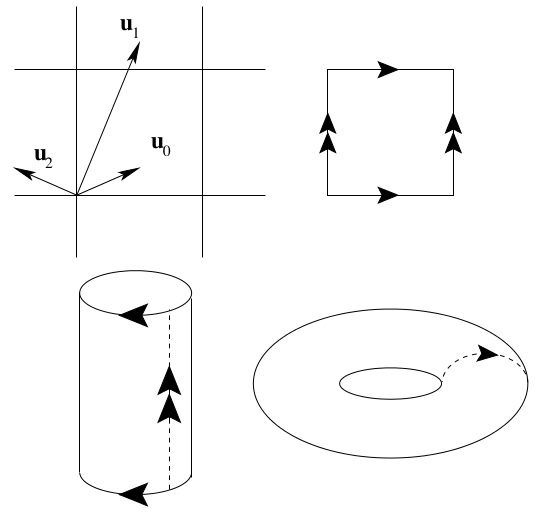
\includegraphics[scale=0.3]{OPspacecrystal.png}
 \caption{The order parameter space for the phonon field on a square lattice. 
Top left: different expressions of $\bv u$ are related by crystal lattice 
vector translation. Top right: $\bv u$ needs to be confined to a periodic 
square, that is, the unit cell. Bottom: gluing together the ends identified by 
periodicity, it becomes clear that the order paramter $\bv u$ lives on a torus. 
Figure credit to Sethna \cite{sethna}.}
\label{OPspacecrystal}
\end{figure}

The order parameter $\bv u$ can wind 
nontrivially along two axes, so we need a vector winding number to classify 
dislocations. These are the Burgers vectors, and they are integer multiples of 
the underlying real-space lattice vectors, just as the winding number in the XY 
system was an integer multiple of $2\pi$, the angular periodicity. Some 
examples of dislocations and their corresponding Burgers vectors are shown in 
Figure \ref{dislocations}.

Now a proper Hamiltonian is needed that takes into account the topological 
structure of the order parameter $\bv u$. The field $\bv u$ is divided into a 
part that trivially traverses the order parameter space, which is labeled 
$\phi$ and a part composed of dislocation energies \cite{2dmelt}.
\begin{multline} \mathcal{H} = \recip{2} \int d^2\br \, \paren{ 2\mu 
\phi_{ij}^2(\br) + \lam \phi_{ii}^2(\br) } - \frac{K}{4\pi} \sum_{i<j} 
b_\mu(\br_i) b_\nu(\br_j)  \left ( \d_{\mu\nu}\log \frac{\abs{\br_i - 
\br_j}}{\a} \right. \\- \left.\frac{(\br_i - 
\br_j)_\mu(\br_i-\br_j)_\nu}{\abs{\br_i-\br_j}^2} \right ) + E_C \sum_i 
\abs{\bv b(\br_i)}^2. \end{multline}
Here, the constant $K = \frac{4\mu(\mu+\lam)}{2\mu+\lam}$, and $E_C$ is the 
core energy of the dislocations. This Hamiltonian bears a resemblance to the 
XY Hamiltonian with vortices, except that the interaction energies of the 
defects depend on their directions. Still, there is a tendency for dislocations 
that are pointing along the same direction to repel from each other, and there 
is a logarithmic potential well that binds two dislocations of opposite Burgers 
vector together. The set of possible Burgers vectors is also subject to the 
condition $\sum_i \bv b_i = 0$, just like in the XY model.

It's clear that the spontaneous generation of dislocation pairs will destroy 
local order. When the temperature becomes high enough, dislocation pairs will 
unbind and roam freely around the sample. Just like the unbinding of 
vortex-antivortex pairs leads to exponential correlation decay, dislocation 
pair unbinding leads to exponential translational order decay. This correlation 
function below the unbinding transition temperature is
\[ \avg{e^{i \bv G \cdot (\bv u(\br) - \bv u(0))}} \sim r^{-\eta(T)}, \qquad 
\eta(T) = \frac{k_BT \abs{\bv G}^2}{4\pi} \frac{3\mu + \lam}{\mu(2\mu+\lam)}.\]
Here, $\bv G$ is any reciprocal lattice vector. The correlation decay 
exponent depends on nonuniversal parameters like the temperature and elastic 
coupling strengths $\lam$ and $\mu$, just as it did in the XY model, but there 
with $J$.

\begin{figure}
 \centering
 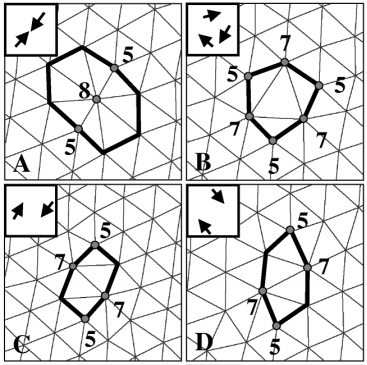
\includegraphics[scale=0.4]{pointdefects.png}
 \caption{Shown here are bound dislocations, and in the top left corners, the 
Burgers vectors associated with the dislocations.}
\label{dislocations}
\end{figure}

From this point, the next step would be to calculate the renormalized elastic 
constants $\lam_R$ and $\mu_R$, as the presence of free dislocations give the 
crystal an avenue by which to relieve applied stress. In this way, dislocations 
are said to reduce the elasticity of materials. To recreate or explain 
sufficiently the renormalization group calculation is beyond my ability, but 
the results due to Kosterlitz and Thouless (taken from \cite{40years}) show 
that the ratio $K$ flows to a universal value as the melting temperature is 
approached:
\beq K_R(T_m^-) = \recip{k_BT_m}\frac{4\mu_R(\mu_R + \lam_R)}{2\mu_R + 
\lam_R} \goto 16\pi.\eeq
Here, the temperature $T_m$ is the temperature at which the system changes from 
power-law translational correlations to exponentially decaying translational 
correlations.

The work of Nelson and Halperin \cite{2dmelt}, and Young \cite{young} extended 
the work of Kosterlitz and Thouless by considering \emph{bond orientational 
order}. Though the presence of dislocations disrupt translational order (Figure 
\ref{disclinations}), they do not disrupt the six-fold orientational order. 
Any path around a dislocation produces zero winding of the bond order. The 
defects responsible for destroying bond orientational order are 
\emph{disclinations}. Two bare disclinations are shown in Figure 
\ref{disclinations}. A disclination core is marked by a lattice site that has 
more or fewer than 6 bonds. Looking closely at Figure \ref{dislocations}, a 
dislocation defect is really a bound state of two oppositely charged 
disclination defects.

\begin{figure}
 \centering
 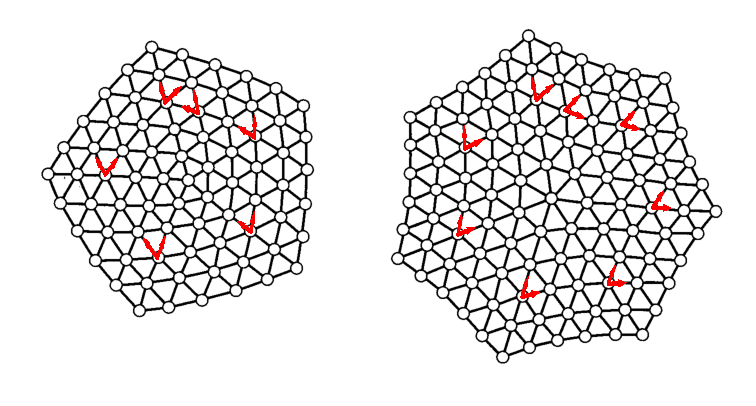
\includegraphics[scale=1.2]{disclinations.eps}
 \caption{Illustrations of bare disclinations in a triangular lattice. Any 
path around the defect core (a site that has more or less than six bonds) 
produces a nonzero winding of the bond orientation. The left shows a 
$+\pi/3$ disclination, and the right shows a $-\pi/3$ disclination. Figure due 
to Chaikin and Lubensky \cite{Chaikin}, arrows added for clarity.}
\label{disclinations}
\end{figure}

The Hamiltonian involving the bond orientational order is identical to the XY 
Hamiltonian, but instead of the fundamental relevant winding numbers being 
$\pm1$, the bond-orientation winding numbers of interest are $\pm1/6$.

The correlation function of interest in this regime of interest is the 
bond-orientational correlation function, or the hexatic correlation function:
\beq \psi_6(\br) = e^{6i\th(\br)},\quad \avg{\psi_6(\br)\psi_6^*(0)} \sim 
r^{-\eta_6(T)}. \eeq

This algebraic decay of bond-orientation correlations in a regime where the 
translational correlations decay exponentially defines the \emph{hexatic 
phase}. This is a liquid-like phase that retains quasi-long range 
orientational order without a definite crystal lattice. From here, because of 
the identification with the XY model Hamiltonian, Nelson, Halperin, and Young 
deduced that the transition from the hexatic phase to the true liquid phase 
takes place by dislocations unbinding into their composite disclination pairs 
which move around the sample and destroy local orientational order. The true 
fluid phase occurs above this second transition temperature and is defined by 
exponentially decaying bond-orientation and translational correlations 
\cite{2dmelt,young}.

\section{Conclusion}
The XY model provided the first system where topological defects in the order 
paramter were shown to participate crucially near the critical point. 
Two-dimensional melting of crystal lattices provides another model with more 
detail that follows the spirit of the XY model calculations. Kosterlitz and 
Thouless's early work on the XY model showed that the transition from quasi-long 
ranged order to disorder was mediated by unbinding of topological defects. 
Nelson, Young and Halperin showed later that topological defects in crystals 
became unbound and mediated the transition from quasi-long range 
translational and then orientational order. The basic theory finds applications 
in superfluid helium films, where topological defects are vortices of 
superfluid flow, in liquid crystals, where the topological defects are also 
dislocations and disclinations, and several other systems \cite{Chaikin}.


\section{Appendix: Calculation of $\eta$ in the XY Model without Vortices}

This appendix is a detailed calculation of the critical exponent $\eta$ in 
the XY model, mostly to prove to myself that I can perform this calculation. 
The Hamiltonian corresponding to our spin variables $\th_i$ on a square lattice 
of spacing $a$ in the quadratic approximation is
\beq \mathcal H = \half{J}\sum_{\langle i,j \rangle} (\th_i - \th_j)^2 \goto 
\frac{J}{2}\int d^2\br \, \paren{\nabla \th(\br)}^2. \eeq
We can apply the Fourier transform:
\beq \th(\br) = \recip{(2\pi)^2} \int d^2\bv k \, e^{-i\Dot kr} \tilde{\th}(\bv 
k), \qquad \mathcal H = \frac{J}{2} \int \frac{d^2\bv k}{(2\pi)^2} \, k^2 
\abs{\tilde{\th}(\bv k)}^2. \eeq
Here, the integral over $\bv k$ is the square Brillouin zone $k_x,k_y\in
[-\pi/a,\pi/a]$. The canonical partition function is then
\beq Z = \int \mathcal{D}\th \, \exp\paren{-\frac{\b J}{2 } \int 
\frac{d^2\bv k}{(2\pi)^2} \, k^2\abs{\tilde{\th}}^2 }.\eeq
This is a Gaussian functional integral which is calculable exactly. If we add a 
term that is linear in $\tilde \th$ that is coupled to some other function 
$\tilde{h}(\bv k)$, then the partition function is
\beq Z(\tilde h) = \int \mathcal{D}\th \, \exp\paren{\recip{2\pi}\int 
\frac{d^2\bv k}{(2\pi)^2} \, \paren{-\frac{\b Jk^2}{2 }\abs{\tilde{\th}}^2 + 
\tilde{h}\tilde{\th}^* }}.\eeq
We can complete the square to compute this Gaussian integral:
\begin{multline} -\frac{\b Jk^2}{2 }\abs{\tilde{\th}}^2 + 
\tilde{h}\tilde{\th}^* = -\half{1} \paren{ \b Jk^2\abs{\tilde{\th}}^2 -
2\tilde{h}\tilde{\th}^* - \frac{1}{\b J k^2} \abs{\tilde{h}}^2} + 
\frac{1}{2 \b J k^2} \abs{\tilde{h}}^2 \\ = -\frac{\b J k^2}{2} 
\abs{\tilde \th - \frac{a}{k\sqrt{\b J}} \tilde h}^2 + \frac{1}{2 \b 
J k^2} \abs{\tilde{h}}^2. \end{multline}
The functional integral integrates over all possible configurations of 
$\tilde{\th}(\bv k)$, so the shift by a function of $\bv k$ does not affect the 
functional integral. What remains is an exponential function of $\tilde h$:
\beq Z(\tilde h) = Z(\tilde h = 0) \exp\paren{ \int \frac{d^2\bv 
k}{(2\pi)^2} \, \frac{1}{2 \b J 
k^2} \abs{\tilde{h}}^2}. \eeq
This is useful now because we are interested in calculating the correlation 
function
\[ \avg{\bv S(\br) \cdot \bv S(0)} = \avg{e^{i(\th(\br) - \th(0))}} = 
\recip{Z(\tilde h = 0)} \int \mathcal{D} \th e^{-\b \mathcal{H} + i\th(\br) - 
i \th(0) }.\]
Here, we can right away substitute the linear function $h(\br') = 
i\paren{\d(\br' -\br) - \d(\br') }$ which is easily expressed in 
Fourier space:
\beq \tilde h(\bv k) = \frac{i}{(2\pi)^2}\, \paren{ e^{i 
\Dot{k}{r}} - 1 }.\eeq
So the correlation function is then
\beq \avg{e^{i(\th(\br) - \th(0))}} = \frac{Z(\tilde h = 0)}{Z(\tilde h = 0)} 
\exp\paren{ \int \frac{d^2\bv k}{(2\pi)^2}\, \frac{1}{2 \b J k^2} 
\paren{2 - 2\cosp{\Dot kr}}} .\eeq
The integral over the Brillouin zone in the exponent is very difficult to solve 
analytically, but for large $r$, Mathematica gives that the leading order term 
is logarithmic in $r$, and the coefficient of the $\log r$ term is $\recip{2\pi 
\b J}$:
\beq \avg{e^{i(\th(\br) - \th(0))}} = e^{\mathrm{const.} - \eta(T)\log(r/a)} = 
C_0 \paren{\frac{r}{a}}^{-\eta(T)}, \quad \eta(T) = \frac{k_BT}{2\pi J}. \eeq
This gives the power-law decay in the absence of vortices which is a good 
approximation at low temperatures.


\bibliography{Final_Project_Refs}
\bibliographystyle{uiuchept}


\end{document}